\section{IDE}
\subsection{Webstorm [M]}
\setauthor{Fabian Maar}
\begin{wrapfigure}{r}{0.3\textwidth}
  \begin{center}
    
\includegraphics[width=0.2\textwidth]{pics/webstorm_logo.png}
   \caption{Webstorm Logo}
  \end{center}
\end{wrapfigure}
\emph{Webstorm} ist eine Entwicklungsumgebung vom Unternehmen JetBrains, die sich auf die Programmiersprache JavaScript spezialisiert hat. Sie wurde besonders für das Arbeiten mit Angular optimiert. Dies zeigt sich durch viele Features, die das Entwickeln von Angular-Projekten erleichtern. So macht es Webstorm möglich, mit nur wenigen Mausklicks eine neue Angular-Dependency oder Komponente zu erstellen. Auch wird die Entwicklungszeit durch intelligente Code-Vervollständigung, Code-Formatierung, einfache Navigation und viele weitere hilfreiche Features deutlich verkürzt. \cite{Webstorm}

\section{UI Prototyping Werkzeug [L]}
Es gab verschiedene Auswahlkriterien für das UI-Prototyping-Werkzeug: 
\begin{compactitem}
  \item flache Lernkurve - Das Werkzeug sollte es ermöglichen, sofort in den Designprozess einzusteigen, ohne neue Konzepte und Arbeitsschritte lernen zu müssen.
  \item komponentenbasiert - Da Angular für die Umsetzung der Single-Page-Application gewählt wurde, sollte das Werkzeug auch komponentenbasiert sein.
  \item Kollaboration - Das Werkzeug sollte es ermöglichen, zusammen Design-Prototypen zu entwickeln und schnelles Feedback einzuholen.
\end{compactitem}

Das Tool \emph{Figma} erfüllte die Auswahlkriterien und wurde für dieses Projekt als UX/UI-Design-Tool gewählt.

\subsection{Figma [L]}
\setauthor{Litzlbauer Lorenz}
\label{ch::technologies::figma}

\begin{wrapfigure}{r}{0.3\textwidth}
  \begin{center}
    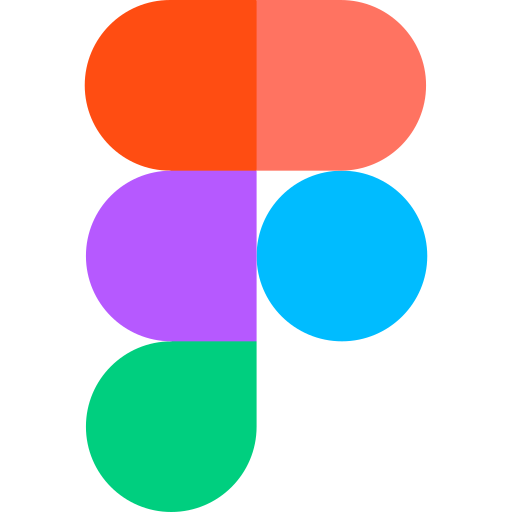
\includegraphics[width=0.2\textwidth]{pics/figma_logo.png}
   \caption{Figma Logo}
  \end{center}
\end{wrapfigure}

Figma ist ein Programm für die Erstellung und Testung von UI und UX Prototypen. Das Programm ist einsteigerfreundlich, denn es hat eine benutzerfreundliche Oberfläche und es gibt viele Tutorials auf der Webseite und von der Figma Community. Figma ist primär eine Web-Applikation, bietet aber auch eine Desktop-Version für macOS und Windows sowie eine mobile Version für iOS und Android an. Figma arbeitet mit mehreren Konzepten, um den Designprozess zu vereinfachen:

\paragraph{Kollaboration}
In Figma können mehrere Personen gleichzeitig auf verschiedenen Geräten designen. Es gibt verschiedene Rollen, wie Zuschauer*in, Kritiker*in oder Mitarbeiter*in. Die Möglichkeiten können genutzt werden um einen*einer Kunden*in in den Designprozess zu involvieren und schon früh Feedback auf das Design bekommen zu können.

\paragraph{Plugins}
Figma hat eine große Community, gibt es ein Feature nicht, kann dieses von der Community im PluginStore als Plugin hinzugefügt werden. Ein Plugin ist eine Software-Erweiterung, welche die Fähigkeiten oder die Features eines Softwareprojektes erweitert.

Für die Design-Prototypen wurde das Plugin \emph{Iconify} verwendet. Dadurch wird  Figma durch eine weitere Oberfläche erweitert. Auf dieser Oberfläche kann nach Icons gesucht und diese Icons direkt im Design verwendet werden.

\paragraph{Assets}
Figma arbeitet mit dem Konzept der Assets. Bereits designte Komponenten können als Assets gespeichert und wiederverwendet werden. Figma legt einen großen Wert auf die Modularität. Beispielsweise können Farben und Pixelgrößen auch als Variablen gesichert werden. Bei einer Veränderung der Variablen wirkt sich diese sofort auf das Design aus.

\section{3D Moddelierung}
\subsection{Cinema4D [M]}
\setauthor{Fabian Maar}
\begin{wrapfigure}{r}{0.3\textwidth}
  \begin{center}
    
\includegraphics[width=0.2\textwidth]{pics/cinema4d_logo.png}
   \caption{Cinema4D Logo}
  \end{center}
\end{wrapfigure}
\emph{Cinema4D} ist ein professionelles Programm des Unternehmens Maxon zur 3D-Modellierung und Animation. Zum einen ist die Software leicht zu bedienen und zum anderen bietet Maxon eine Vielzahl an Tutorials und Anleitungen. Im Unterschied zu anderen 3D-Programmen wie Autodesk Maya, führt Cinema4D schnell zu einem anwendbaren Wissen. Aufgrund der intuitiven Benutzeroberfläche ist das Programm sowohl für Einsteiger als auch für Profis geeignet. \cite{Cinema4D}

\begin{figure} [h t]
    \centering
    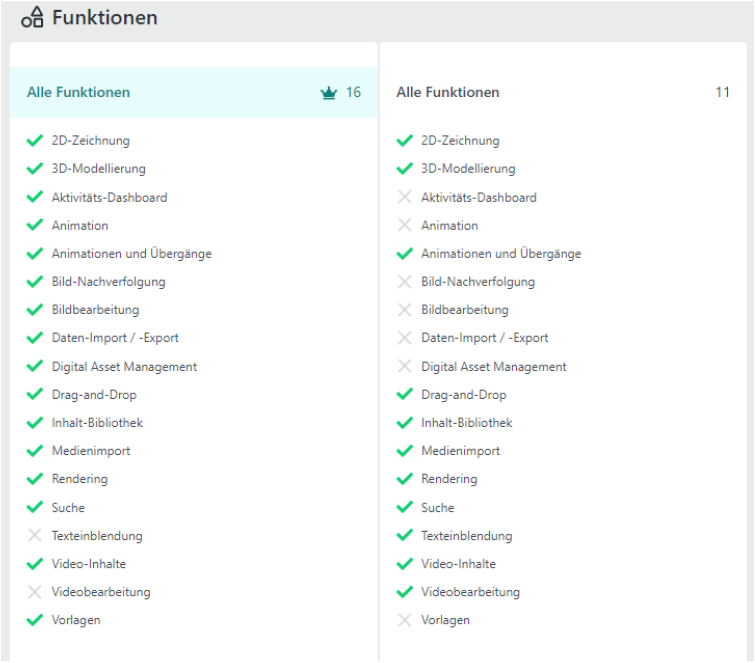
\includegraphics[scale=0.7]{pics/c4d-vs-maya.PNG}
    \caption{Cinema4D vs Maya \cite{C4DvsMaya}}
    \label{fig:tech:front:c4d-vs-maya}
  \end{figure}

Ein weiterer wichtiger Aspekt ist die Unterstützung des Exportes von GLTF-Files anzuführen. GLTF ist das Dateiformat, das genutzt wird, um ein 3D-Modell in der Three.js Szene zu laden. Da alternative 3D-Programme wie zum Beispiel Blender diese Exportmöglichkeit nicht anbieten, war Cinema 4D die gewählte Option für die 3D-Modellierung.   

\section{Package Manager [L]}
\subsection{NPM - Node Package Manager [L]}
Der Node Package Manager ist ein Softwareverwaltungstool zum Downloaden, Aktualisieren, Veröffentlichen und Verwalten von OpenSource-Programmen in der NodeJs-Umgebung. \cite{whatNpm} \cite{AboutNpm}


